\chapter{$HH\rightarrow 4b$ Results}\label{ch:hh4b-results}

\red{0p07 und m5 training, mit diesen fertigen training, only cuts optimieren}

This chapter presents the extracted cross-section limits for the $HH\rightarrow 4b$ analysis and explorations in limit setting optimization. To test on any \ktwov hypothesis a linear combination of available samples is employed as explained and validated in \ref{sec:linear_combination}.




\begin{landscape}
    \begin{figure}
        \centering
        \subfigure[]{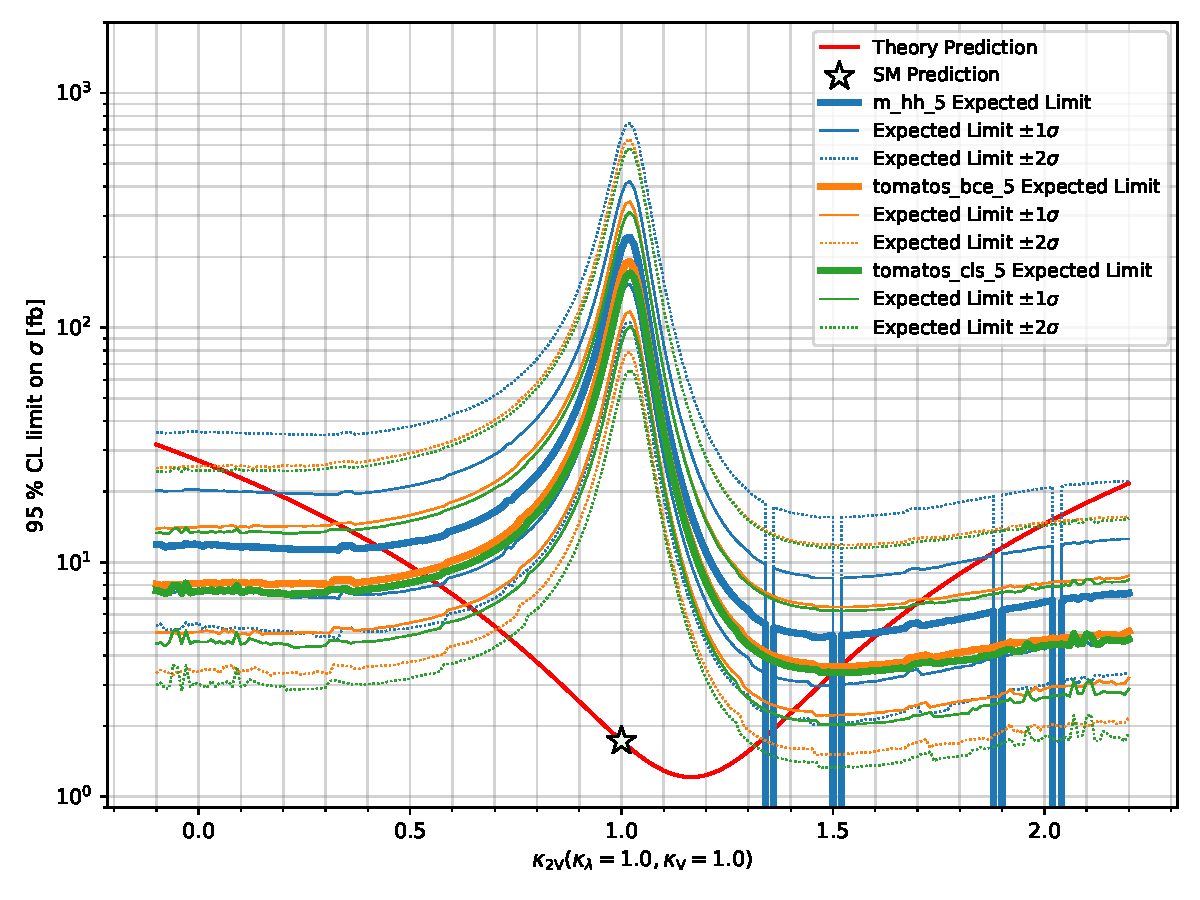
\includegraphics[width=.7\textwidth]{k2v_scan_limits_overlay_vbf_cut}}
        \subfigure[]{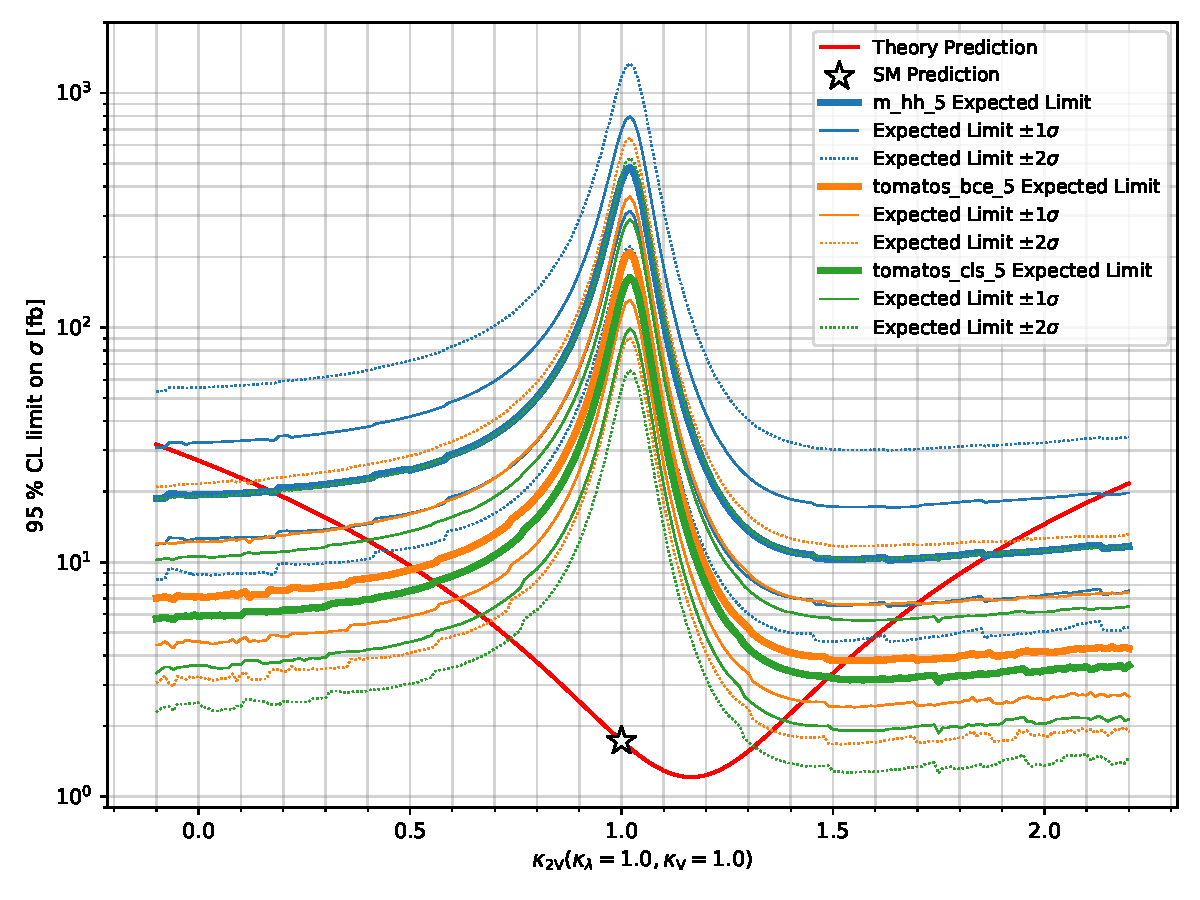
\includegraphics[width=.7\textwidth]{k2v_scan_limits_overlay_no_vbf_cut}}
        \caption[]{\red{(a) with vbf cut (b) without vbf cut, still unhappy with these plots, probably only show expected, and say as can be seen in figures sowieso that the limits are similar between all of them. y-axis should be cls}}
        \label{fig:k2v_scan_limits_overlay}
    \end{figure}
\end{landscape}


go back, correct objects,  orrect neos, correct bkg estimate, put all the stuff from this to methodology

% m_hh, tomatos_bce, tomatos_cls
% k2v=1, k2v=0
% vbf_cut, no_vbf_cut
% pre and post fit 
% uncertainties--> uncertainties chapter
% pulls, already in ranking
% what does hh4b paper say to ttbar background


where does the twist happen to decide to use tomatos? show fit results first, if the decisions actually comes at last, then maybe here in the argumentation too...
show one whole iteration of a fit for sm and k2v=0

show plot with signal, ggf, vbf for sm and k2v=0 with and without vbf cut?

even though mhh benefits from the vbf cut, the overall performance is always better for the \ac{ml} models and even improves upon removing the vbf cut
does removing the vbf cut actually reduce the CLs upper limit by a factor of $\sim 2$

unblinded plot
fit plots
ranking
scan
show bin studies?
\red{in theory could turn on binning, by figuring how to disable binning parameters so the opimization cant find gradients anymore
    degeneracy argument… hat nichts gebracht etc. nn should learn which bin, oder erwähnen, show plots of the nn score with/without}

how to frame it, show improvement comparison to naive training?, whole scan or k2v0 enough

we are better without vbf cut
% The analysis has very limited sensitivity to constrain 𝜅𝜆 as it’s in the boosted regime while 𝜅𝜆 is sensitive959
% in the region of lower 𝑚HH . And VBF topology with two forward jets is required thus ggF signal which960
% contributes most to 𝜅𝜆 is suppressed. A combination with the resolved analysis [44] can present more961
% stringent constraint on 𝜅𝜆.

correlation matrix usw in anhang



\red{Pulls allow one to estimate how well a model fits the data. A pull is a value computed for each data bin. It is given by (observed - predicted) / standard-deviation. If the model is correct, the expectation value of each pull is zero and its variance is one in the asymptotic limit of infinite samples. Under these conditions, the chi-square statistic is computed from the sum of pulls squared has a known probability distribution if the model is correct. It therefore serves as a goodness-of-fit statistic.}